\chapter{Desenvolvimento}

No capítulo anterior foram mostradas as características, os pontos fortes de cada tecnologia, e também os motivos para sua escolha. Nesse capítulo será descrito a especificação do projeto para o sistema proposto, seu funcionamento e estrutura.

O projeto consiste basicamente, na implementação de uma solução que possibilite a criação de cursos em vídeos com elementos de questões interativas integrado com um sistema de gestão de aprendizado [\autoref{sec:lms}] por meio do \textit{LTI} [\autoref{sec:lti}].

O funcionamento do sistema é baseado no modelo cliente/servidor, permitindo que o cliente realize solicitações ao servidor, que então envia os resultados de volta ao cliente, como pode ser vista na figura~\ref{fig:comunicacao-cliente-servidor}.

\begin{figure}[h]
    \centering
    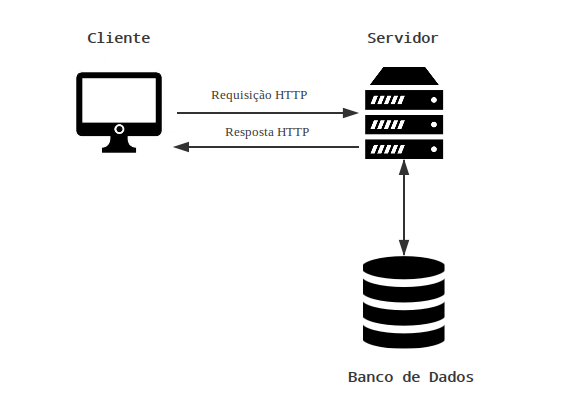
\includegraphics[keepaspectratio=true,scale=0.7]{figuras/comunicacao_cliente_servidor.png}
    \caption{Ilustração da comunicação cliente/servidor}
    \label{fig:comunicacao-cliente-servidor}
\end{figure}

O desenvolvimento foi dividido em três camadas que são: Camada de Negócio, Camada do Banco de Dados e camada de Apresentação, que serão descritas a seguir.

\section{Camada do Banco de Dados}

O banco de dados utilizado foi o \textit{Mysql} (\autoref{sec:mysql}). A modelo conceitual de dados está representado na seguinte DER (Diagrama Entidade-Relacionamento) figura~\ref{fig:diagrama-er}, que é um diagrama que define as entidades de um sistema, e como elas estão relacionadas.

\begin{figure}[h]
    \centering
    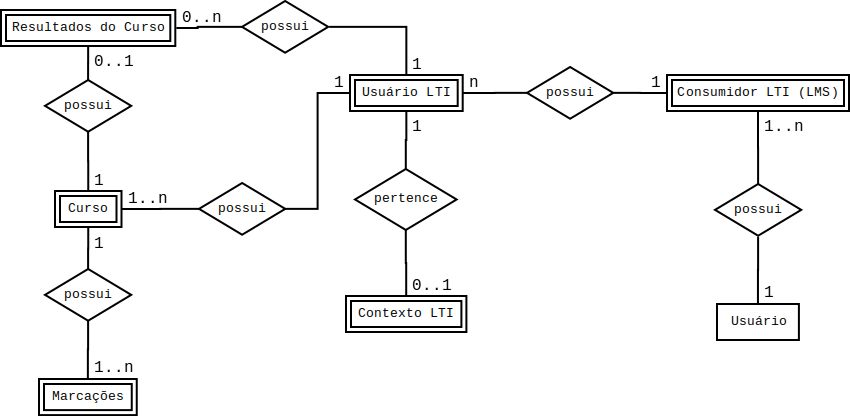
\includegraphics[keepaspectratio=true,scale=0.4]{figuras/der_video_interativo.png}
    \caption{Diagrama ER (Entidade-Relacionamento) do banco de dados.}
    \label{fig:diagrama-er}
\end{figure}

\subsection{Mapeamento objeto-relacional}

A partir da elaboração do DER, mostrando a visão geral do relacionamento entre os dados, foi possível definir as classes de Mapeamento objeto-relacional (\textit{ORM}), criados usando como base o textit{Eloquent ORM} fornecido pelo \textit{framework Laravel}, as classes definidas são representadas na figura~\ref{fig:diagrama_classe_eloquent}

\begin{figure}[htpb]
  \centering
  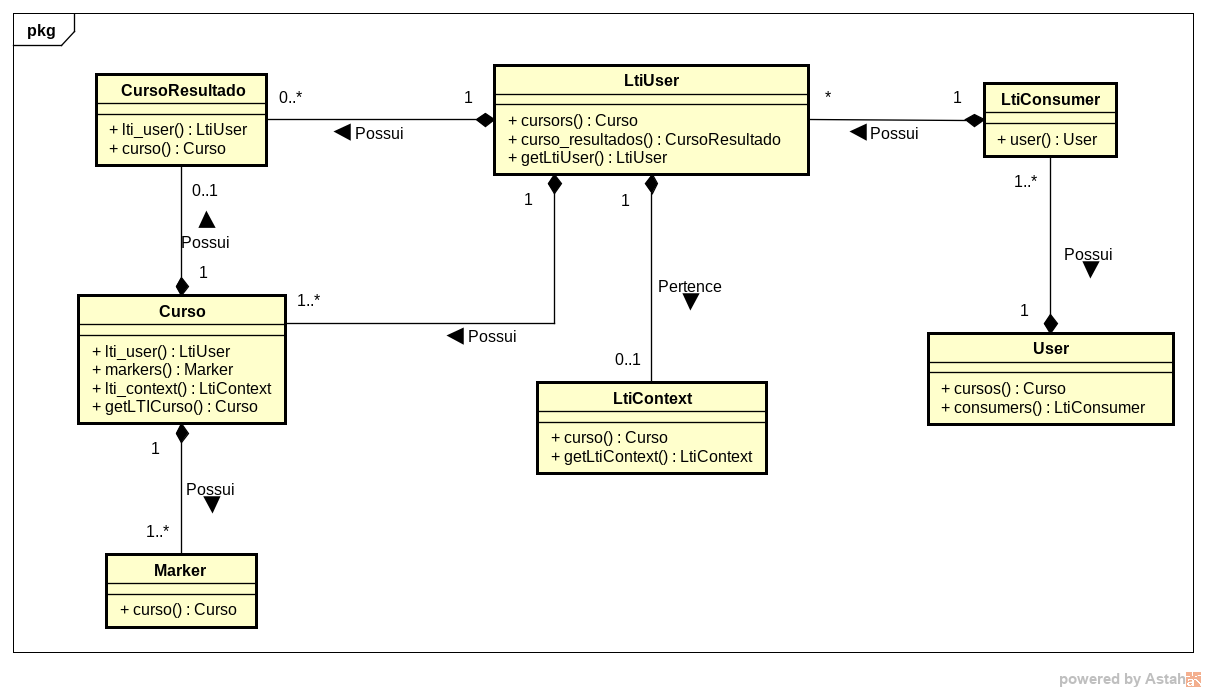
\includegraphics[width=1.0\linewidth]{figuras/diagrama_classe_eloquent.png}
  \caption{Representação das classes \textit{ORM}}
  \label{fig:diagrama_classe_eloquent}
\end{figure}

\section{Camada de Negócio}

Esta camada foi desenvolvida utilizando o servidor \textit{Apache}, descrito na \autoref{sec:apache}, na linguagem \textit{PHP} (\autoref{sec:php}), e para facilitar e estruturar o desenvolvimento, foi usado o \textit{framework Laravel}, que como descrito na \autoref{sec:laravel} é baseado no padrão arquitetural \textit{MVC} (\autoref{sec:mvc}) que tem como objetivo criar independência e divisão de responsabilidades das partes que envolvem o sistema.

\begin{figure}[h]
    \centering
    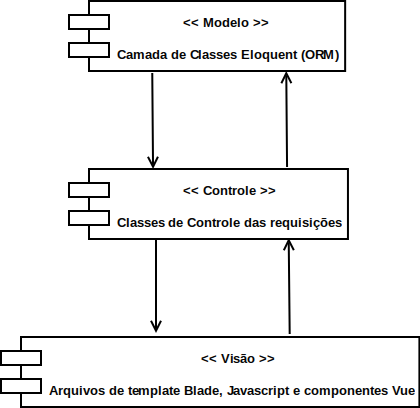
\includegraphics[keepaspectratio=true,scale=0.45]{figuras/diagrama_mvc.png}
    \caption{Implementação da arquitetura \textit{MVC} no projeto}
    \label{fig:diagrama-mvc}
\end{figure}

Na camada do servidor, a parte mais importante do \textit{MVC} são os \textit{Controllers}, que recebem as requisições do cliente e os \textit{Models} que realizam a comunicação com a camada de Banco de Dados.

A separação dos \textit{controllers} do projeto, pode ser visto na tabela~\ref{tbl:controllers}.

\begin{table}[htp]
\begin{tabular}{|p{.20\textwidth}|p{.80\textwidth}|}
    \hline \textbf{Controller}        & \textbf{Descrição} \\
    \hline \textit{AuthController}    &
        Esse \textit{controller} tem o papel de gerenciar as autenticações simples do sistema, criar e validar as contas. O \textit{controller} foi gerado pelo \textit{Laravel} que contém um modulo de autenticação, mais foi necessário modifica-lo para adicionar a criação da chave do consumidor da integração do \textit{LTI}, ou seja, quando um usuário novo cria uma conta, o sistema precisa gerar também uma chave que será usada para se conectar ao \textit{LMS}.
                                     \\
    \hline \textit{HomeController}    &
        Tem a simples função de criar uma rota para a página inicial do sistema.
                                     \\
    \hline \textit{CursosController}  &
        Tem responsabilidade de tratar as requisições \textit{REST} enviadas pelo cliente para o cadastro e realização do curso.
                                     \\
    \hline \textit{LtiController}     &
        As requisições \textit{LTI} feitas pelo \textit{LMS} passam primeiro por esse \textit{controller}, na ação \textit{launch} (lançamento) onde é feita a comunicação com a \textit{API} do \textit{LTI}.
                                     \\
    \hline 
    \end{tabular} 
    \caption{Tabela com a descrição dos controladores do projeto.}
    \label{tbl:controllers}
\end{table}

Os modelos (\textit{models}), são os objetos que proporcionam a comunicação com o banco de dados, tais como consultas e persistência dos dados. O acesso ao banco de dados é feita utilizando a \textit{ORM Eloquent} que como mostrado na \autoref{sec:laravel} consiste em uma \textit{API} de abstração na comunicação com o banco, proporcionando também a compatibilidade dos \textit{drivers} utilizados, ou seja, o mesmo código funcionará para qualquer banco de dados suportado pelo \textit{framework}.

\begin{figure}[htpb]
  \centering
  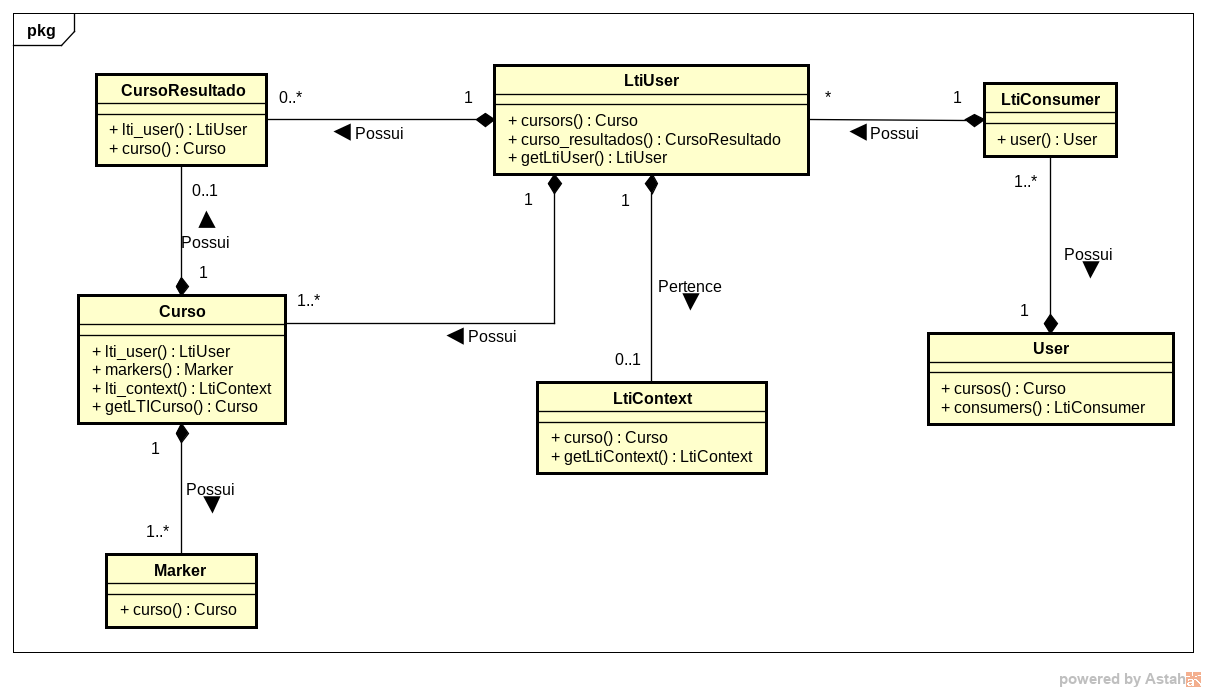
\includegraphics[width=1.0\linewidth]{figuras/diagrama_classe_eloquent.png}
  \caption{Diagrama de Classe, representando os \textit{models eloquent}.}
  \label{fig:diagrama_classe_eloquent}
\end{figure}

\subsection{Integração LTI}
\label{sec:integracao}

A integração do sistema com o \textit{LTI} foi feita utilizando uma \textit{API} desenvolvida por \textit{Stephen Vickers}, que depois de algumas pesquisas foi a biblioteca que melhor atendeu os requisitos de versão do \textit{LTI} 1.1+ que tem a funcionalidade de retornar as notas ao \textit{TC}, podendo ser encontrada em \url{http://projects.oscelot.org/gf/project/php-basic-lti/}.

Para realizar a integração foram usadas as seguintes classes da \textit{API};

\begin{itemize}
    \item \textit{LTI\_Tool\_Provider}: Classe usada pra representar um \textit{Tool Provider}, realiza a conexão com o \textit{LMS} por meio do método \textit{handle\_request()}, e guarda suas informações para inserir no banco de dados.
    \item \textit{LTI\_Tool\_Consumer}: Representa um \textit{Tool Consumer} ou seja quem está se conectando com a \textit{TP}.
    \item \textit{LTI\_Resource\_Link}: Representa o link de recurso (\textit{resource link}) entre o \textit{TP} e o \textit{TC}.
    \item \textit{LTI\_Data\_Connector}: Classe abstrata para a persistência dos objetos \textit{LTI} listados acima.
    \item \textit{LTI\_User}: Representa um um objeto de usuário \textit{LTI}.
    \item \textit{LTI\_Outcome}: Contem as operações de retorno da nota para o \textit{TC}.
    \item \textit{LTI\_Data\_Connector\_pdo}: Implementação da classe abstrata \textit{LTI\_Data\_Connector}, para a conexão com o banco de dados utilizando a extensão do \textit{PHP} \ac{PDO}.
\end{itemize}

\begin{sloppypar}
  O primeiro passo da implementação foi criar uma classe que herdava de \textit{LTI\_Tool\_Provider}, seguindo as especificações da \textit{API}, então foi criada a classe Video\_Interativo\_LTI\_Tool\_Provider e implementado o método \textit{onLaunch} que é chamado quando a requisição \textit{LTI} é finalizada, no método foram criadas variáveis de sessão usadas pelo sistema para identificar o usuário.
\end{sloppypar}

No \textit{LtiController} foi criado a \textit{action launch} que é o ponto inicial da aplicação chamada pelo \textit{TC}, utilizando o endereço http://endereço-do-tool-provider/lti/launch. Na \textit{action} foi criada uma instância de \textit{Video\_Interativo\_LTI\_Tool\_Provider} e então foi chamado o método \textit{handle\_request()} provido pela \textit{API} que autentica o usuário, verificando se os dados recebidos estão válidos por meio do \textit{OAuth}, e se a requisição é de fato um pedido \textit{HTTP LTI}. Na mesma \textit{action} e feito a verificação se o usuário é professor ou aluno (dados recebidos pelo \textit{TC}), e então é feito o redirecionamento de página dependendo do seu papel, o professor é redirecionado para uma página onde ele pode criar o curso, e o aluno para uma tela onde ele pode realizar o curso, caso o mesmo já tenha sido criado pelo docente. O fluxo básico da integração pode ser visto no diagrama de sequencia na figura~\ref{fig:diagrama-sequencia-lti}

\begin{figure}[htbp]
    \centering
    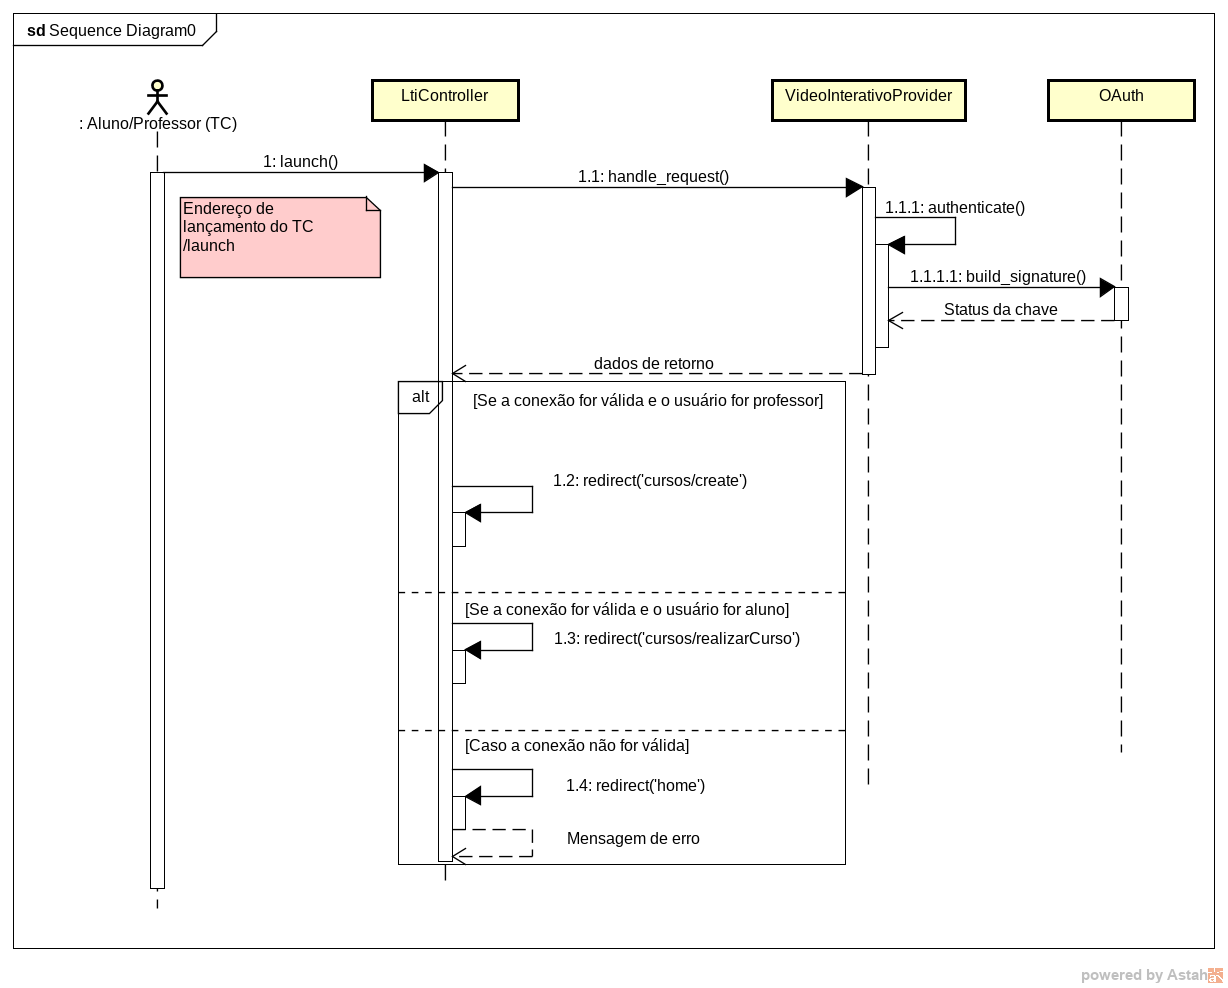
\includegraphics[keepaspectratio=true,scale=0.45]{figuras/diagrama_sequencia_lti.png}
    \caption{Diagrama de Sequência da integração}
    \label{fig:diagrama-sequencia-lti}
\end{figure}

Quando o usuário é um professor e ele entra na tela de criação do curso, o sistema primeiro verifica se algum curso já foi criado para o \textit{resource\_id} enviado pelo \textit{TC}, caso já tenha sido criado, o professor é redirecionado para uma tela com as informações dos alunos que fizeram o curso, caso contrario é dado a permissão de criar o curso, que quando finalizado gerará um vinculo com o \textit{resource\_id} no sistema. No caso do aluno, quando entra na tela de realizar o curso, também é verificado se já existe um curso vinculado, caso não exista é mostrado somente uma mensagem, avisando que o professor do curso ainda não criou a atividade.

É importante lembrar que quando o sistema está tratando uma conexão \textit{LTI} em vez da autenticação comum, é usada uma verificação de autenticidade segura por meio do \textit{OAuth}, então o sistema de autenticação do \textit{framework} não é valido nesse caso, como visto na figura~\ref{fig:diagrama-sequencia-autenticacao} a verificação é baseada em checar se o usuário (retirado da tabela \textit{users}) está na sessão. 

\begin{figure}[htbp]
    \centering
    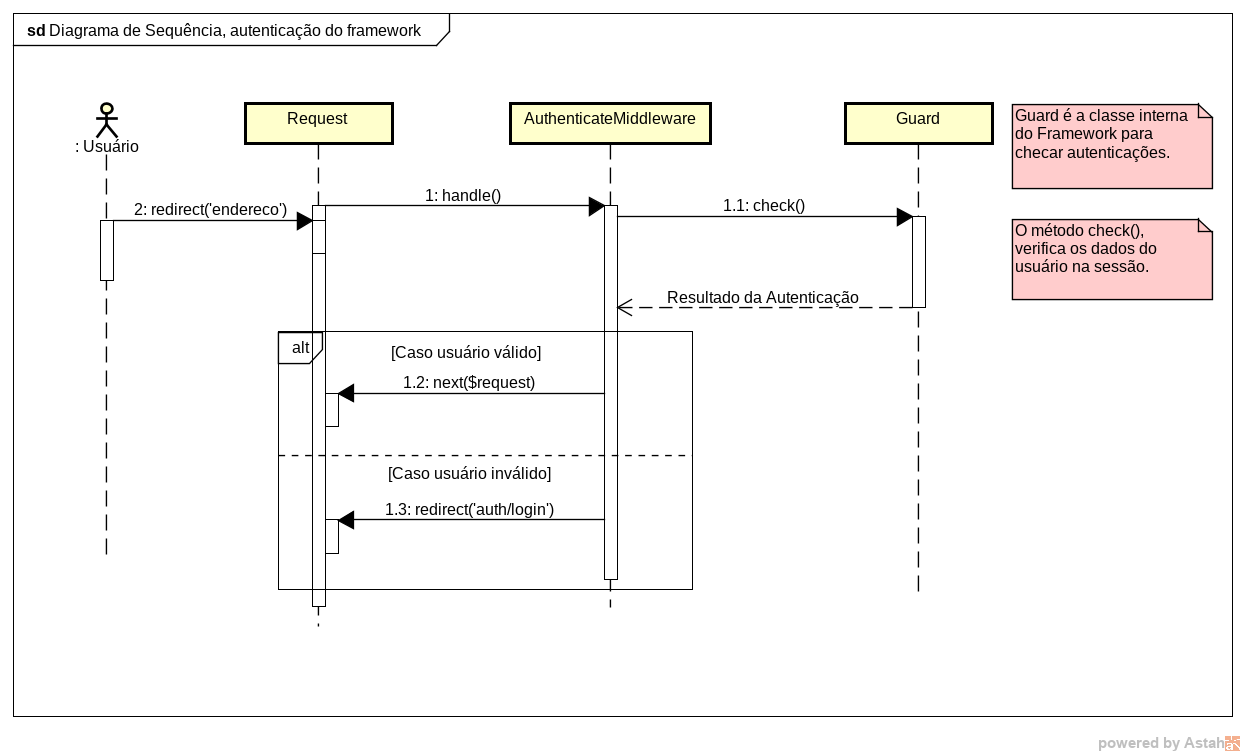
\includegraphics[keepaspectratio=true,scale=0.45]{figuras/diagrama_sequencia_autenticacao.png}
    \caption{Diagrama de Sequência representando a autenticação do \textit{framework}}
    \label{fig:diagrama-sequencia-autenticacao}
\end{figure}

Por esse motivo foi criado um \textit{HTTP Middleware}\footnote{\url{http://laravel.com/docs/master/middleware}}, que é uma implementação conveniente do \textit{framework} que nos permite filtrar as requisições de forma centralizada.

O \textit{Middleware} criado se chama \textit{LtiCheckMiddleware} sua função é verificar se a conexão é válida, checando os dados da sessão e os comparando com os dados do banco de dados, checando assim a consistência da requisição, caso a verificação falhe o sistema fecha a conexão do usuário é retorna um erro, avisando que é necessário utilizar um Sistema de Gestão de Aprendizagem para executar essa função, caso contrario a requisição continua, a visualização desse processo pode ser visto no diagrama~\ref{fig:diagrama-sequencia-autenticacao-lti}

\begin{figure}[htbp]
    \centering
    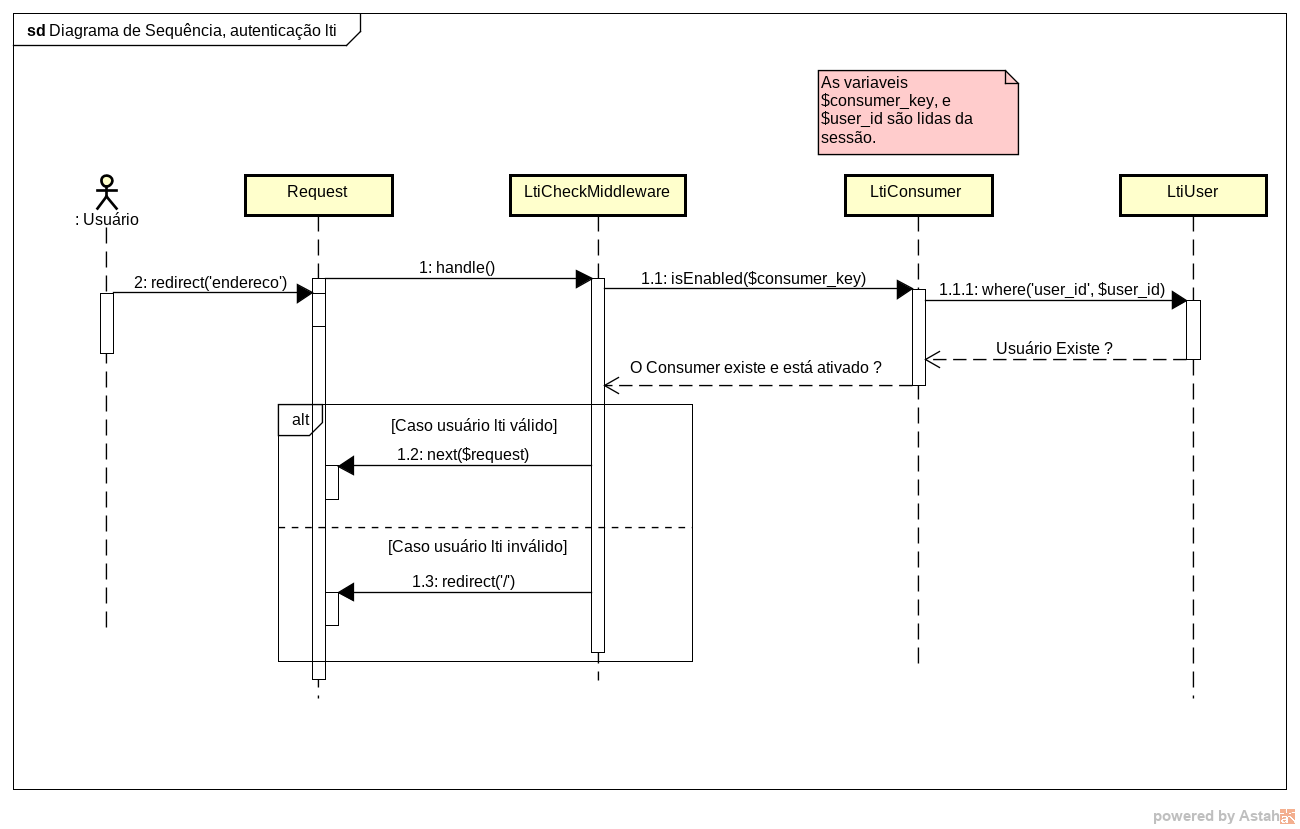
\includegraphics[keepaspectratio=true,scale=0.45]{figuras/diagrama_sequencia_autenticacao_lti.png}
    \caption{Diagrama de Sequência representando a autenticação \textit{LTI}}
    \label{fig:diagrama-sequencia-autenticacao-lti}
\end{figure}

Para utilizar esse \textit{middleware} é preciso primeiramente dizer ao \textit{framework} que todas as requisições que envolvem \textit{lti} necessitam passar por esse filtro, para isso foi necessário definir um grupo de rotas como pode ser visto no código~\ref{lst:laravel-routing-lti}.

\begin{listing}
    \phpfile{codigos/lti-middleware.txt}
    \caption{Mapeamento das rotas do \textit{Laravel} para o grupo do \textit{middleware lti}}
    \label{lst:laravel-routing-lti}
\end{listing}

O retorno das notas \textit{Outcome}, foi um processo simples utilizando a biblioteca, que retorna para o \textit{TC} um \textit{XML} contendo os dados do contexto, usuário, recurso e nota, então \textit{TC} verifica os dados e então modifica a nota do aluno, um exemplo de uso utilizando \textit{PHP} pode ser visto no código~\ref{lst:lti-outcome}.

\begin{listing}
    \phpfile{codigos/lti-outcome.txt}
    \caption{Exemplo de envio de nota para o \textit{Tool Consumer}}
    \label{lst:lti-outcome}
\end{listing}


\subsection{Dificuldades da integração}

As maiores dificuldades da integração foram causados pela biblioteca \textit{PHP} escolhida, por ter um código um pouco antigo, foi necessário fazer algumas modificações nela para se adequar melhor com o \textit{framework} e com a arquitetura de desenvolvimento.

A primeiro problema encontrado, foi que todas as classes da \textit{API} estavam centralizados em um só arquivo \textit{PHP} o \textit{LTI\_Tool\_Provider}, gerando uma dificuldade no processo de depuração e até na leitura e entendimento do código, então foi necessário separar cada classe em seu arquivo seguindo o guia de estilo de codificação \textit{PSR-2} (\textit{PHP Coding Standarts})\footnote{\textit{PHP Coding Standarts Versão 2} \url{http://www.php-fig.org/psr/psr-2/pt-br/}}.

Depois de separado os arquivos, foi percebido que os arquivos eram chamados por meio da função \textit{include} do \textit{PHP} fugindo do padrão e também dificultando seu uso no \textit{framework laravel} que segue o \textit{PSR-2} e todas as classes precisam estar dentro de pacotes (\textit{namespaces}), e necessitam ser chamadas usando a declaração \textit{use}. Então foi feita essa refatoração do código da biblioteca colocando-as no \textit{namespace} \textit{Lti}, permitindo assim que o \textit{framework} a utilize como uma classe comum.

As conexões de banco de dados da biblioteca são feitas de forma direta com consultas \textit{SQL}, diferente da \textit{ORM Eloquent}, por esse motivo foi necessário fazer uma ponte da interface \textit{pdo} \textit{laravel} com o classe de conexão do \textit{LTI} a \textit{LTI\_Data\_Connector\_pdo} de forma que não seja necessário definir duas vezes os dados de conexão com o banco de dados, evitando duplicidade.

\section{Camada de Apresentação}

A camada de apresentação do projeto foi feita utilizando basicamente \textit{HTML, CSS e Javascript} com a ajuda de algumas bibliotecas e ferramentas já detalhadas no referência teórico.

As \textit{views} foram criadas utilizando o sistema de \textit{templates blade} do \textit{Laravel} simplificando o uso de \textit{HTML} e \textit{PHP} em um mesmo arquivo e a definição do \textit{layout} do site. Por exemplo, foi criado um \textit{layout} chamado \textit{master.blade.php} que inclui o cabeçalho e o rodapé da pagina, dessa forma todas as paginas que usam esse mesmo \textit{layout} só precisam estendê-lo como mostra o exemplo no código~\ref{lst:blade-template}. Dessa forma não foi necessário duplicar o cabeçalho e rodapé da página em cada \textit{view}.

\begin{listing}
    \begin{phpcode}
        @extends('master')
        @section('title', 'Título da Página')
        
        @section('content')
        // Conteudo da pagina aqui
        @stop
    \end{phpcode}
    \caption{Exemplo do \textit{Template Blade}}
    \label{lst:blade-template}
\end{listing}

As interações com a página, criação do curso e a realização do curso pelo aluno, foram feitas utilizando \textit{Javascript}, mais especificamente foram usadas as bibliotecas \textit{jQuery} (\autoref{sec:jquery}) e \textit{Vue.js} (\autoref{sec:vuejs}).

Como explicado na seção~\autoref{sec:browserify} o \textit{Browserify} foi utilizado para unir todos os \textit{scripts javascripts} do projeto, e também para permitir o uso de \textit{require} que funciona como a declaração \textit{use} do \textit{PHP}. Para poder unir o código de forma automatizada foi usado o \textit{Gulp.JS} (\autoref{sec:gulp}), criando nele uma tarefa que será executada toda vez que o comando \textit{gulp} for executado na pasta do projeto por meio de um terminal.

\begin{listing}
    \begin{jscode}
            // Cria uma tarefa que executa o browserify no arquivo deps.js
            mix.browserify("deps.js", {
                debug: false,
                noparse: ['jquery', 'ckeditor', 'materialize', 'videojs'], // Opções do Browserify
                output: "public/js/", // Pasta de Saída do javascript compilado
            });
        conteúdo...
    \end{jscode}
      \caption{Exemplo de uso do \textit{Browserify + Gulp}}
      \label{lst:browserify-gulp}
\end{listing}

O \textit{deps.js} é um arquivo que guarda todas as dependências do projeto por meio do \textit{require}, nele são chamadas as bibliotecas \textit{Vue, jQuery, jQuery-UI, Video.JS, CKEDITOR (editor de texto em js) entre outros}, o arquivo compilado e chamado no \textit{master.blade.php} no bloco de \textit{scripts}.

\subsection{Desenvolvimento da interface de Vídeo Interativo}

Na criação da interface foi usado o \textit{Vue} que usa o padrão arquitetural \textit{MVVM} (\autoref{sec:mvvm}) e a biblioteca utilizada para a execução e controle do vídeo foi o \textit{Video.js} (\autoref{sec:videojs}).

Infelizmente o \textit{videojs} não suporta vídeos do \textit{Youtube} por padrão, por isso foi necessário o uso de um \textit{plugin} para o \textit{video.js} chamado \textit{videojs-youtube}, criado por Benoit Tremblay, o \textit{plugin} pode ser encontrado nesse repositório do \textit{github} \url{https://github.com/eXon/videojs-youtube}.

O primeiro passo da implementação foi entender como o \textit{Video.JS} funcionava, e estudar sua \textit{API} para poder escutar eventos do vídeo, como por exemplo, mudança de tempo, quando o vídeo parou e quando ele iniciou. Também foi necessário receber informações do vídeo, como o tempo atual do vídeo em segundos.

Após o entendimento do \textit{videojs}, suas funções foram integradas com o \textit{vue.js} por meio da criação de um componente \textit{videojs.vue}, que encapsula as funcionalidades do \textit{player} permitindo seu reuso.

As marcações são as partes mais importantes do desenvolvimento da interatividade com o vídeo, uma marcação (\textit{Marker}) é representada por um objeto \textit{javascript} contendo informações como:
\begin{itemize}
    \item Chave de Identificação da marcação.
    \item Tempo de ativação em segundos.
    \item Tipo da marcação.
\end{itemize}

Quando uma marcação é criada, é gerado um objeto com as informações citadas acima e então ele é inserido em uma \textit{array} na instância \textit{curso} do \textit{Vue}. Na classe \textit{curso} foi criada uma função que escuta o evento de mudança de tempo do vídeo e a cada segundo, é realizado um laço na \textit{array} de \textit{markers} onde é verificado, se o segundo atual é igual ao tempo definido em uma das marcações, quando o tempo é igual a marcação é ativada, o tipo dela é verificado, e então é mostrado para o usuário um componente em um painel referente ao tipo, como por exemplo, um componente de \quotes{Questão Múltipla Escolha}, esse fluxo pode ser visualizado em um diagrama de maquina de estado na figura~\ref{fig:diagrama-maquina-estado}.
\newpage

\begin{figure}[H]
    \centering
    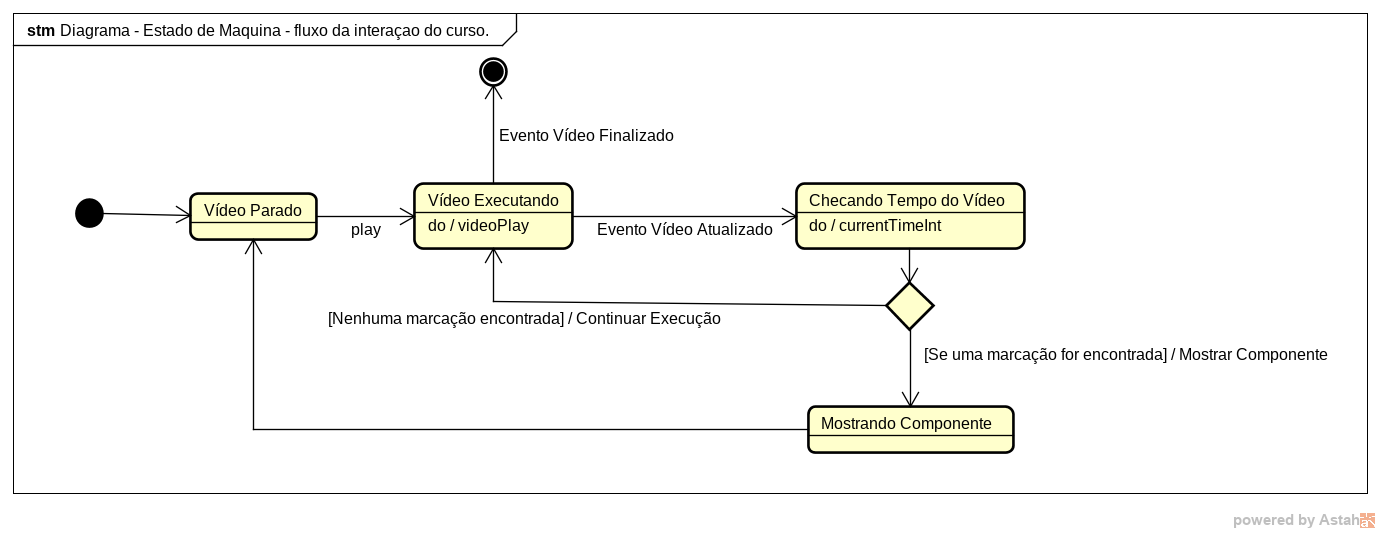
\includegraphics[keepaspectratio=true,scale=0.43]{figuras/diagrama_estado_maquina.png}
    \caption{Diagrama Maquina de estado ilustrando o processo do vídeo interativo}
    \label{fig:diagrama-maquina-estado}
\end{figure}

Caso o usuário for um professor é dado a ele a permissão de editar os dados dessa marcação, como modificar o titulo, adicionar/remover questões. Se o usuário for um aluno o componente filtra as ações que ele pode executar, deixando somente a possibilidade de responder essas questões.

\subsubsection{Telas do Sistema}

Nessa seção serão apresentadas algumas telas do sistema e sua funcionalidade.

A tela apresentada na figura~\ref{fig:tela-sistema-1}, a seguir, representa a página inicial na visão de um professor conectado por um \textit{TC}, onde ele pode inserir um endereço do vídeo do \textit{youtube}. Ao clicar em \quotes{Começar}, é automaticamente mostrado a seguinte tela~\ref{fig:tela-sistema-2}

\begin{figure}[h]
    \centering
    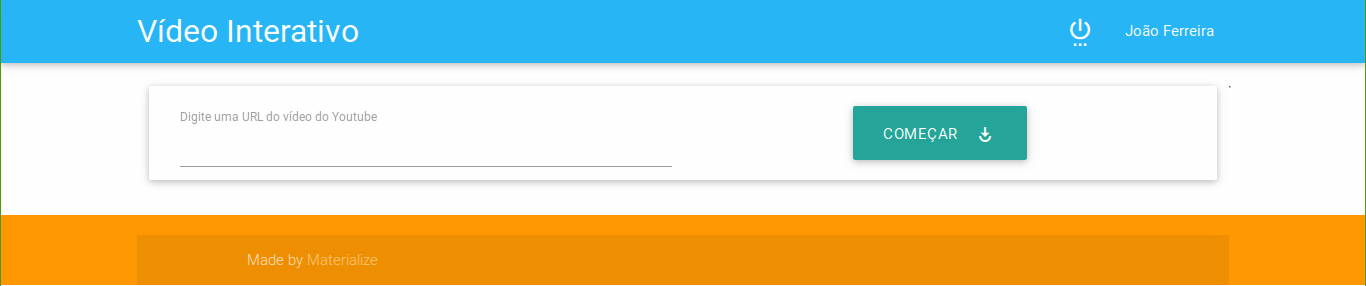
\includegraphics[keepaspectratio=true,scale=0.31]{figuras/tela_sistema_1.png}
    \caption{Tela de inicio do sistema, visão do professor.}
    \label{fig:tela-sistema-1}
\end{figure}

\begin{figure}[h]
    \centering
    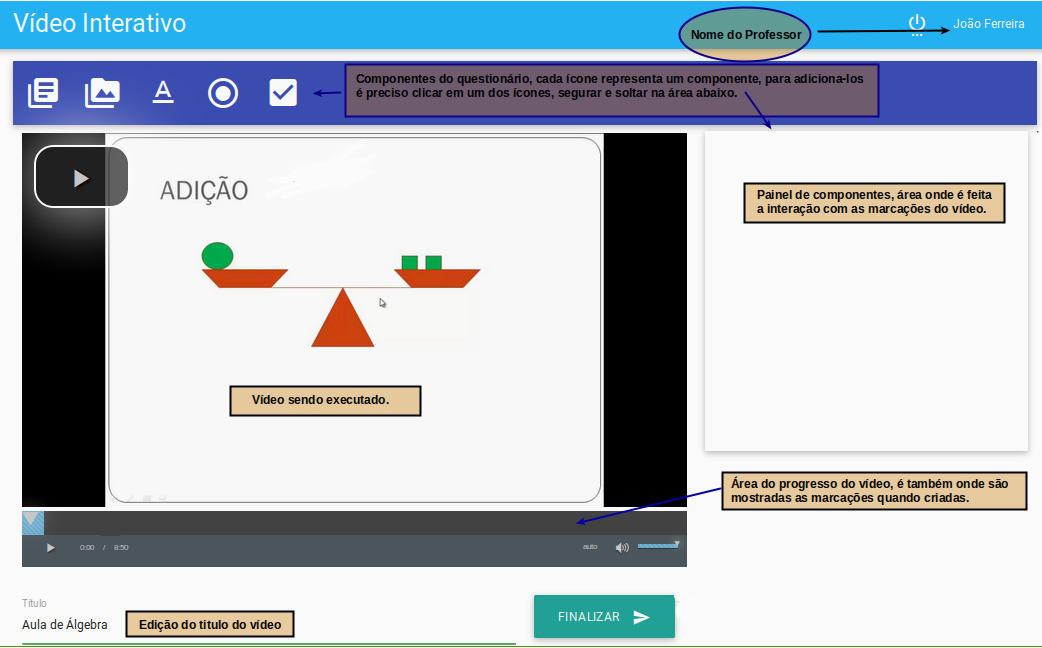
\includegraphics[keepaspectratio=true,scale=0.4]{figuras/tela_sistema_2.png}
    \caption{Tela de criação do vídeo, visão do professor.}
    \label{fig:tela-sistema-2}
\end{figure}

Quando um componente é adicionado ao painel, ele é automaticamente adicionado ao painel, e também é criado uma marcação no tempo atual do vídeo, como pode ser visto na figura~\ref{fig:tela-sistema-3}

\begin{figure}[h]
    \centering
    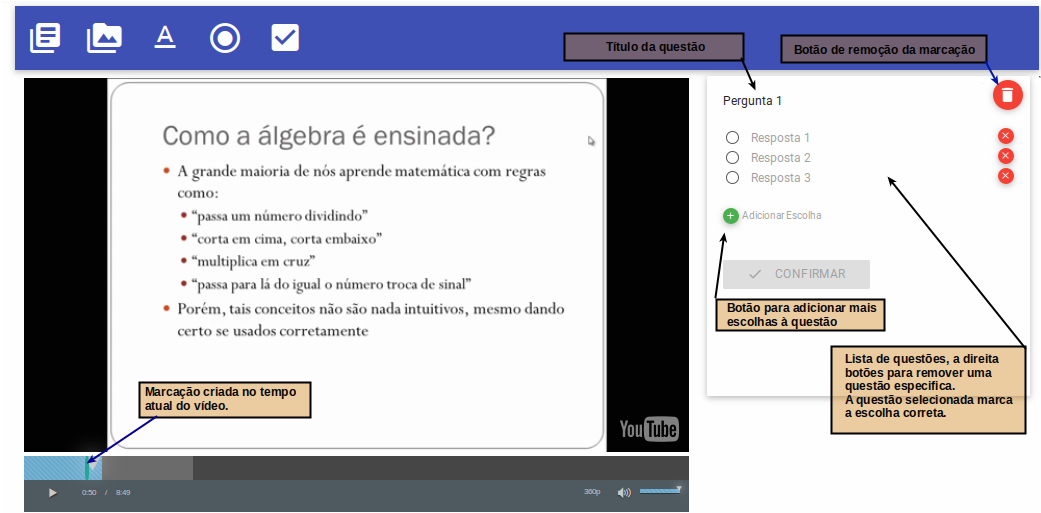
\includegraphics[keepaspectratio=true,scale=0.4]{figuras/tela_sistema_3.png}
    \caption{Tela de criação do vídeo, visão do professor parte 2.}
    \label{fig:tela-sistema-3}
\end{figure}

Já a tela do aluno é semelhante a do professor, com exceção da remoção dos componentes de edição, e a adição do botão de confirmar que verifica se a questão está correta, como visto na figura~\ref{fig:tela-sistema-4}

\begin{figure}[htbp]
    \centering
    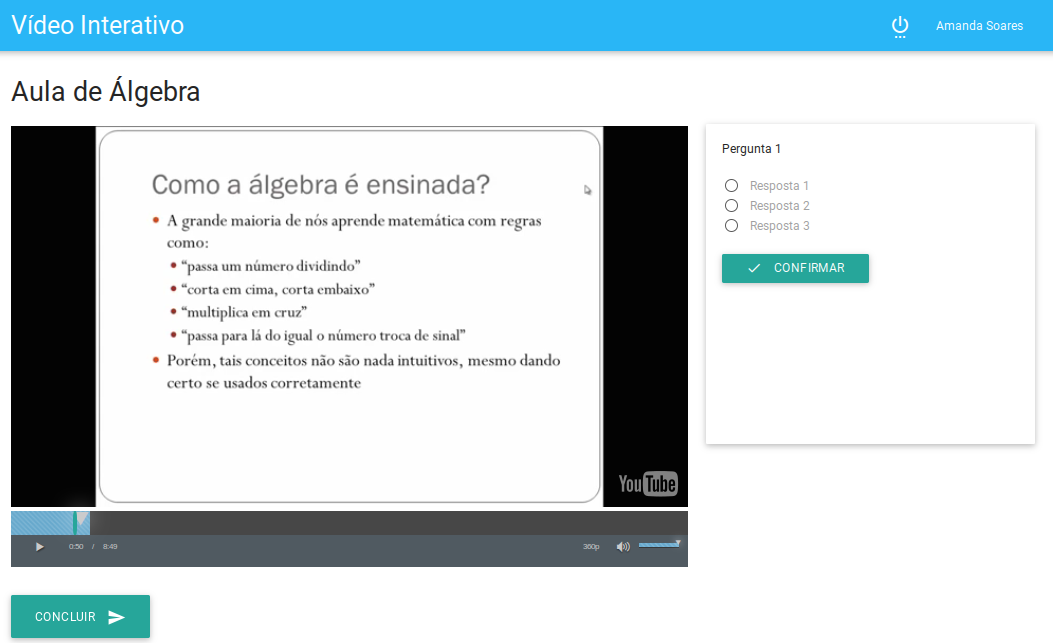
\includegraphics[keepaspectratio=true,scale=0.4]{figuras/tela_sistema_4.png}
    \caption{Tela realização do curso, visão do aluno.}
    \label{fig:tela-sistema-4}
\end{figure}
